\section{Experimental Results}

To evaluate our content-driven reputation, we considered two Wikipedias:
%
\begin{itemize}

\item The Italian Wikipedia, consisting of 154,621 articles and 714,280
  {\em filtered\/} revisions; we used a snapshot dated December~11, 2005.
\item The French Wikipedia, consisting of 536,930 articles and
  4,837,243 {\em filtered\/} revisions; we used a snapshot dated
  October~14, 2006.

\end{itemize}
%
In both Wikipedias, we studied only \texttt{NS\_MAIN} pages, which
correspond to ordinary articles (other pages are used as comment
pages, or have other specialized purposes).
Moreover, to allow the accurate computation of our quality
measures which require multiple judges,
we used only revisions that occurred before October~31, 2005 for
the Italian Wikipedia, and before July~31, 2006 for the French one.
Our algorithms for computing content-driven reputation depend on the
value of six parameters, as mentioned earlier.
We determined values for these parameters by searching the parameter
space to optimize the coefficient of constraint $\constrainte$, using the Italian
Wikipedia as a training set; the values we determined are:
%
\begin{align*}
   \coeffrep      & = 13.08
  & \coeffpunish   & = 19.09
  & \lengthexp     & = 0.60   \\
   \slack         & = 2.20
  & \coefftext     & = 0.60
  & \coeffmaxrep   & = 22026
\end{align*}

Figure~\ref{fig:user-breakdown-by-rep} provides a breakdown of
the amount of edits and text additions performed, according to the
reputation of the author.
We find an essentially bimodal distribution:
the overwhelming majority of revisions are authored by the
lowest and highest reputation users in the system.
Note the similarity to the results of Chapter~\ref{ch:contrib},
especially Figures~\ref{fig-revs-quality} and~\ref{fig-user-quality};
we again see a bimodal distribution with an immediate drop-off beyond
the lowest reputation, and an upwards trend for frequency as we move
towards the higher end of the reputation spectrum.
We believe that this might reflect the bimodal behavior of the
community; many users tend to make only a small number of edits, and a few users
contribute a great deal (see Figure~\ref{fig-hist-numedits}).


\begin{figure}
\begin{center}
%GNUPLOT: LaTeX picture with Postscript
\begin{picture}(0,0)%
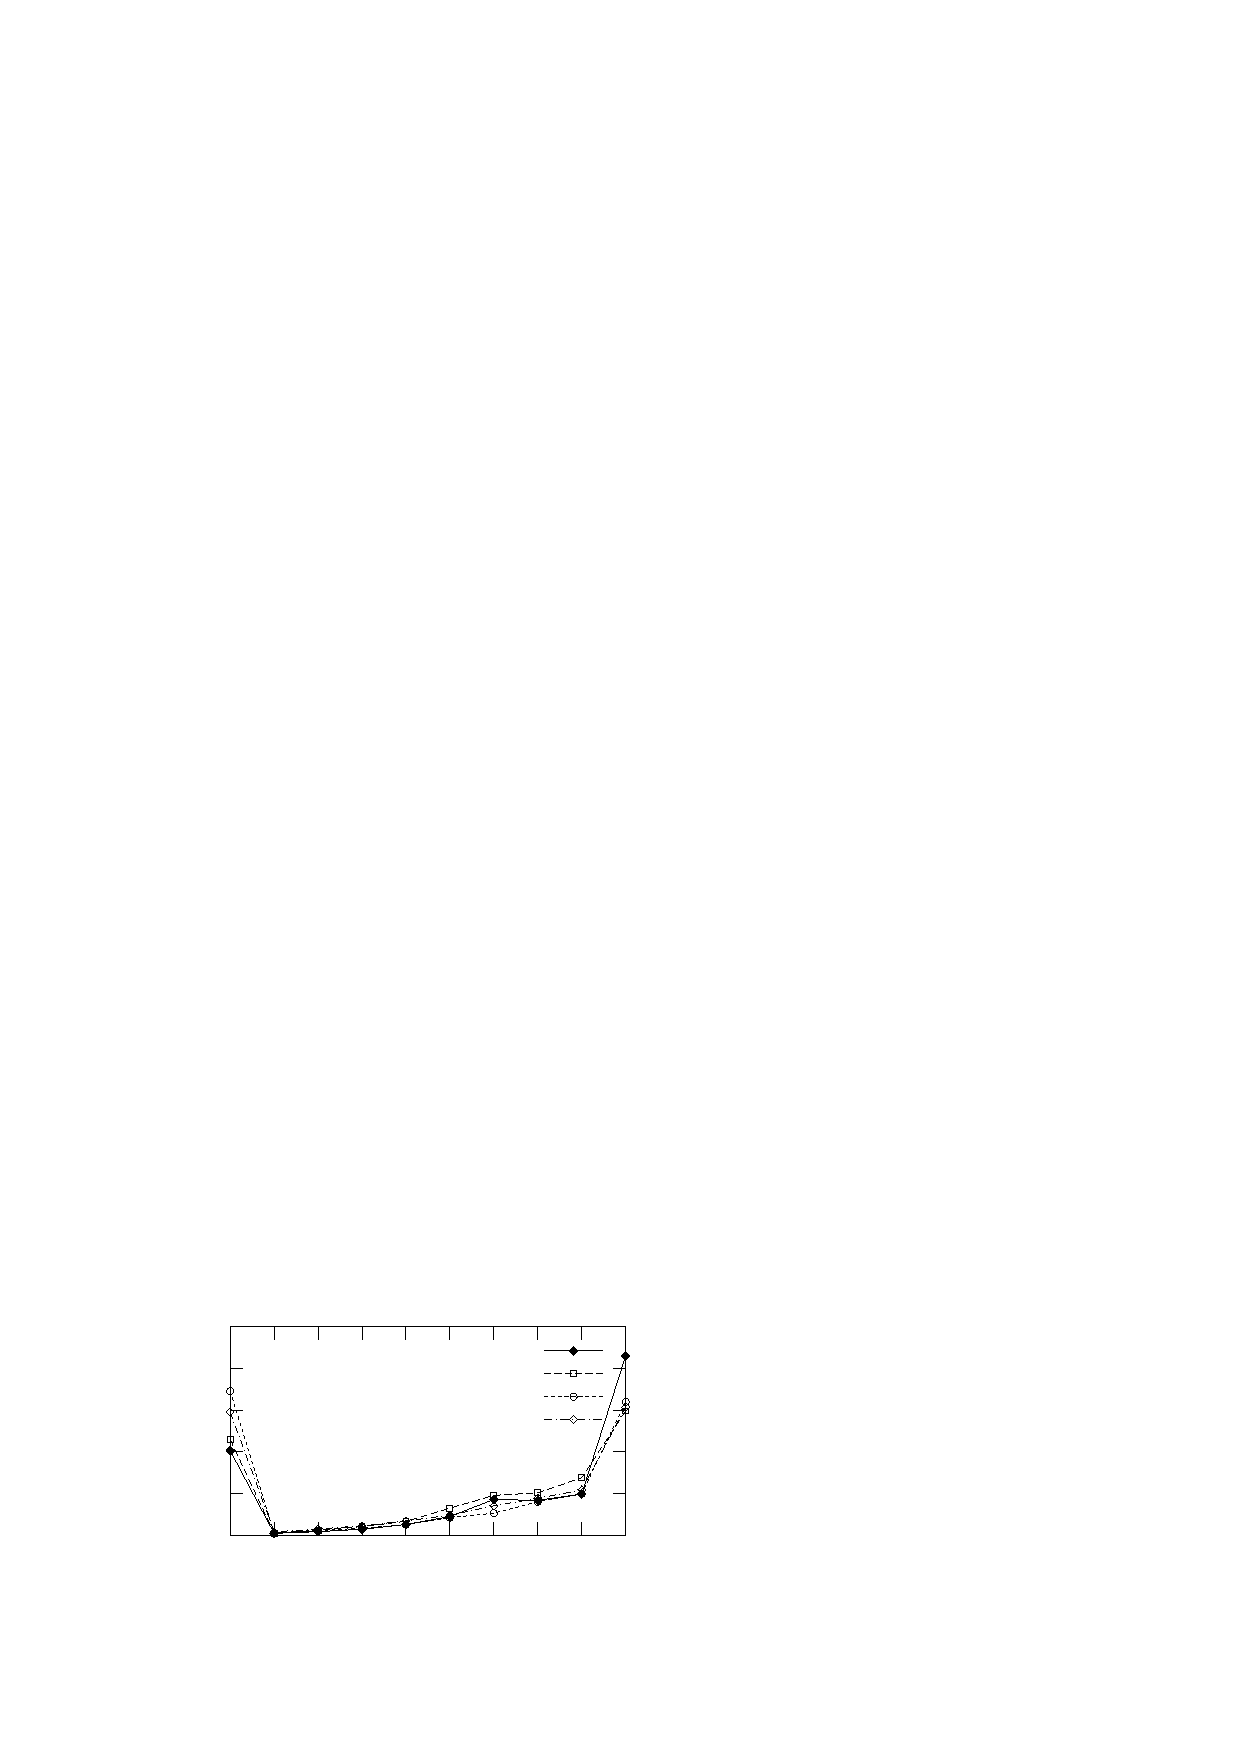
\includegraphics{part-J10-rep/userrep}%
\end{picture}%
\begingroup
\setlength{\unitlength}{0.0200bp}%
\begin{picture}(12240,7200)(0,0)%
\put(1650,1650){\makebox(0,0)[r]{\strut{} 0\%}}%
\put(1650,2650){\makebox(0,0)[r]{\strut{}10\%}}%
\put(1650,3650){\makebox(0,0)[r]{\strut{}20\%}}%
\put(1650,4650){\makebox(0,0)[r]{\strut{}30\%}}%
\put(1650,5650){\makebox(0,0)[r]{\strut{}40\%}}%
\put(1650,6650){\makebox(0,0)[r]{\strut{}50\%}}%
\put(1925,1100){\makebox(0,0){\strut{} 0}}%
\put(2979,1100){\makebox(0,0){\strut{} 1}}%
\put(4034,1100){\makebox(0,0){\strut{} 2}}%
\put(5088,1100){\makebox(0,0){\strut{} 3}}%
\put(6143,1100){\makebox(0,0){\strut{} 4}}%
\put(7197,1100){\makebox(0,0){\strut{} 5}}%
\put(8252,1100){\makebox(0,0){\strut{} 6}}%
\put(9306,1100){\makebox(0,0){\strut{} 7}}%
\put(10361,1100){\makebox(0,0){\strut{} 8}}%
\put(11415,1100){\makebox(0,0){\strut{} 9}}%
\put(6670,275){\makebox(0,0){\strut{}log (1 + reputation)}}%
\put(9190,6075){\makebox(0,0)[r]{\strut{}Italian Wikipedia, edit}}%
\put(9190,5525){\makebox(0,0)[r]{\strut{}Italian Wikipedia, text}}%
\put(9190,4975){\makebox(0,0)[r]{\strut{}French Wikipedia, edit}}%
\put(9190,4425){\makebox(0,0)[r]{\strut{}French Wikipedia, text}}%
\end{picture}%
\endgroup
\endinput

\end{center}
\caption[Text and edit contributions by reputation]{%
  Percentage of text and edit contributed to the
  Italian and French Wikipedias, according to author reputation.
  The data includes anonymous authors.}
\label{fig:user-breakdown-by-rep}
\end{figure}


\subsection{Precision and Recall}

We analyzed the Italian and French Wikipedias using the
parameter values discovered by our optimization procedure.
The results are summarized in Table~\ref{tbl:summary-results}.
The results are better for the larger French Wikipedia; in particular,
our reputation's ability to predict short-lived edits is better on the
French than on the Italian Wikipedias.
We are not sure whether this depends on different dynamics in the two
Wikipedias, or whether it is due to the greater age (and size) of the
French Wikipedia.
We see that edits performed by low-reputation authors are four times
as likely as the average to be short-lived.

\begin{sidewaystable}[tp]
\begin{center}
\begin{tabular}{|r||c|c||c|c||c|c||c|c|} \hline
 & \multicolumn{2}{|c||}{Precision}
 & \multicolumn{2}{|c||}{Recall}
 & \multicolumn{2}{|c||}{Boost}
 & \multicolumn{2}{|c|}{Coeff.\ of constr.} \\
 & Edit & Text & Edit & Text  & Edit & Text & Edit & Text \\
 & $\prece$ & $\prect$ & $\recalle$ & $\recallt$ & $\booste$ & $\boostt$
 & $\constrainte$ & $\constraintt$ \\[0.5ex] \hline
\textbf{Excluding anonymous authors: \quad} & & & & & & & & \\
\qquad French Wikipedia          & 23.92\% &  5.85\% & 32.24\% & 37.80\% & $4.21\times$ & $4.51\times$ &  7.33 &  6.29 \\
\qquad Italian Wikipedia         & 14.15\% &  3.94\% & 19.39\% & 38.69\% & $4.03\times$ & $5.83\times$ &  3.35 &  7.17 \\ \hline
\textbf{Including anonymous authors: \quad} & & & & & & & & \\
\qquad French Wikipedia          & 48.94\% & 19.01\% & 82.86\% & 90.42\% & $2.35\times$ & $2.97\times$ & 25.29 & 23.00 \\
\qquad Italian Wikipedia         & 30.57\% &  7.64\% & 71.29\% & 84.09\% & $3.43\times$ & $3.58\times$ & 19.83 & 17.49 \\ \hline
\end{tabular}
\end{center}
\caption[Evaluation of WikiTrust on Italian and French Wikipedias]
  {Summary of the performance of content-driven reputation for
  the Italian and French Wikipedias.}
\label{tbl:summary-results}
\end{sidewaystable}


\subsection{Manual Annotation}

To investigate how many of the edits had a short life due to bad quality,
we asked a group of seven volunteers to rate revisions made to the
Italian Wikipedia.
We selected the revisions to be ranked so that they contained
representatives of all 4 combinations of high/low reputation author,
and high/low longevity.
We asked the volunteers to rate the revisions with $+1$ (good),
$0$ (neutral), and $-1$ (bad); in total, 680 revisions
were ranked.
The results, summarized in Table~\ref{tbl:human}, are striking.
Of the short-lived edits performed by low-reputation users, fully
66\% were judged bad.
On the other hand, less than 19\% of the short-lived edits performed by
high-reputation users were judged bad.
We analyzed in detail the relationship between user reputation, and
the percentage of short-lived text and edits that users considered bad.
Using these results, we computed the approximate recall factors on the
Italian Wikipedia of content-driven reputation for {\em bad\/} edits,
as judged by users, rather than short-lived ones:
%
\begin{itemize}

\item The recall for short-lived edits that are judged to be bad is over
  49\%.

\item The recall for short-lived text that is judged to be bad is over
  79\%.

\end{itemize}
%
These results clearly indicate that our content-driven reputation is a
very effective tool for spotting, at the moment they are introduced,
bad contributions that will later be undone.
There is some margin of error in this data, as our basis for
evaluation is a small number of manually-rated revisions, and human
judgement on the same revisions often contained discrepancies.

The fact that so few of the short-lived edits performed by
high-reputation authors were judged to be of bad quality points to the
fact that edits can be undone for reasons unrelated to quality.
Many Wikipedia articles deal with current events; edits to those
articles are undone regularly, even though they may be of good
quality.
Our algorithms do not treat in any special way current-events pages.
Other Wikipedia edits are administrative in nature, flagging pages that
need work or formatting; when these flags are removed, we classify it
as text deletion.
Furthermore, our algorithms do not track text across articles, so that
when text is moved from one article to another, it is classified as
deleted from the source article.

From Table~\ref{tbl:summary-results}, we note that the precision is
low, by search standards.
Our problem, however, is a prediction problem, not a retrieval
problem, and thus it is intrinsically different.
The group of authors with low reputation includes many authors who are
good contributors, but who are new to the Wikipedia, so that they have
not had time yet to build up their reputation.


\begin{table}
\begin{center}
\begin{tabular}{|r|c|c|} \hline
\qquad \qquad Reputation & Judged bad & Judged good \\ \hline
\multicolumn{1}{|l|}{Short-lived edits: \qquad \quad} & & \\[1ex]
   Low [0.0--0.2]   &    66  \% &    19 \% \\
Normal [0.2--1.0]   &    16  \% &    68 \% \\ \hline
\multicolumn{1}{|l|}{Short-lived text: \qquad \quad} & & \\[1ex]
   Low [0.0--0.2]   &    74  \% &    13 \% \\
Normal [0.2--1.0]   &    14  \% &    85 \% \\ \hline
\end{tabular}
\end{center}
\caption[Performance of WikiTrust compared to manual annotation]
  {User ranking of short-lived edits and text, as a
  function of author reputation, for the Italian Wikipedia.
  We presented edit differences to a test group of users,
  and asked users to rate whether the edit was good or bad.
  In square brackets, we give the
  interval where the normalized value $\log(1+r) / \log (1 +
  \coeffmaxrep)$ of a reputation $r$ falls.  The precentages do not
  add to 100\%, because users could also rank changes as ``neutral''.}
\label{tbl:human}
\end{table}

\subsection{Comparison with Edit-Count Reputation}

\begin{sidewaystable}
\begin{center}
\begin{tabular}{|l||c|c||c|c||c|c||c|c|} \hline
 & \multicolumn{2}{|c||}{Precision}
 & \multicolumn{2}{|c||}{Recall}
 & \multicolumn{2}{|c||}{Boost}
 & \multicolumn{2}{|c|}{Coeff.\ of constr.} \\
 & Edit & Text & Edit & Text  & Edit & Text & Edit & Text \\
 & $\prece$ & $\prect$ & $\recalle$ & $\recallt$ & $\booste$ & $\boostt$
 & $\constrainte$ & $\constraintt$ \\[0.5ex] \hline
\textbf{Italian Wikipedia:} & & & & & & & & \\
\qquad Content-driven reputation & 14.15 &  3.94 & 19.39 & 38.69 & 4.03 & 5.83 & 3.35 & 7.17 \\
\qquad Edit count as reputation  & 11.50 &  3.32 & 19.09 & 39.52 & 3.27 & 4.91 & 2.53 & 6.35 \\ \hline
\textbf{French Wikipedia:} & & & & & & & & \\
\qquad Content-driven reputation & 23.92 &  5.85 & 32.24 & 37.80 & 4.21 & 4.51 & 7.33 & 6.29 \\
\qquad Edit count as reputation &  21.62 &  5.63 & 28.30 & 37.92 & 3.81 & 4.34 & 5.61 & 6.08 \\ \hline
\end{tabular}
\end{center}
\caption[Performance of WikiTrust compared to edit count]
  {Summary of the performance of content-driven reputation over
  the Italian and French Wikipedias. All data are expressed as
  percentages. Anonymous authors are not included in the comparison.
  Precision is the probability that the text or edit longevity is low,
  given that the reputation is low.
  Recall is the probability that the reputation is low, given
  that the text or edit longevity is low.}
\label{tbl:comparison-with-count}
\end{sidewaystable}

We compared the performance of our content-driven reputation to
another basic form of reputation: edit count.
It is commonly believed that, as Wikipedia authors gain experience
(through revision comments, talk pages, and reading articles on
Wikipedia standards), the quality of their submissions goes
up.\footnote{See~\cite{Halfaker2011} for an analysis that refutes
this assumption, however.}
Hence, it is reasonable to take edit count, that is, the number of
edits performed, as a form of reputation.
We compare the performance of edit count, and of content-driven
reputation, in Table~\ref{tbl:comparison-with-count}.
The comparison does not include anonymous authors, as we do not have a
meaningful notion of edit-count for them.
According to our metrics, content-driven reputation
performs slightly better than edit-count reputation on both the Italian
and French Wikipedias.

We believe that one reason edit-count based reputation performs well
in our measurements is that authors, after performing edits that are
often criticized and reverted, commonly either give up their identity
in favor of a ``fresh'' one, thus zeroing their edit-count reputation
and ``punishing'' themselves, or stop contributing to the Wikipedia
altogether.\footnote{This is consistent with the conclusions presented
in~\cite{Halfaker2011}.}
However, we believe that the good performance of edit count is an
artifact, due to the fact that edit count is applied to an
already-existing history of contributions.
Were it announced that edit count is the chosen notion of reputation,
authors would most likely modify their behavior in a way that both
rendered edit count useless, and damaged the Wikipedia.
For instance, it is likely that, were edit count the measure of
reputation, authors would adopt strategies (and automated robots) for
performing very many unneeded edits to the Wikipedia, causing
instability and damage.
In other words, edit count as reputation measure has very little
prescriptive value that would benefit the Wikipedia.
In contrast, we believe our content-driven reputation, by prizing
long-lasting edits and content, would encourage constructive behavior
on the part of the authors.

\subsection{Text Age and Author Reputation as Trust Criteria}

The age of text in the Wikipedia is often considered an
indicator of text trustworthiness, the idea being that text that has
been part of an article for a longer time has been vetted by more
contributors, and thus, it is more likely to be correct~\cite{Cross2006}.
We were interested in testing the hypothesis that author reputation,
in addition to text age, can be a useful indicator of
trustworthiness, especially for text that has just been added to a
page, and thus that has not yet been vetted by other contributors.
Let {\em fresh text\/} be the text that has just been inserted in a
Wikipedia article.
We considered all text that is fresh in all the Italian
Wikipedia, and we measured that 3.87~\% of this fresh text is deleted
in the next revision.  In other words,
$\Pr(\mbox{deleted}\mid\mbox{fresh}) = 0.0387$.
We then repeated the measurement for text that is both fresh, and is
due to a low-reputation author: 6.36~\% of it was deleted in the next
revision, or
$\Pr(\mbox{deleted}\mid\mbox{fresh and low-reputation}) = 0.0636$.
This indicates that author reputation is a useful factor in predicting
the survival probability of fresh text, if not directly its
trustworthiness.
Indeed, as remarked above, since text can be deleted for a number of
reasons aside from bad quality, author reputation is most likely a
better indicator of trustworthiness than these figures indicate.
We investigate a method for computing the ``reputation of text'' that
is based on the ideas presented here in~\cite{Adler2008b}.


